\documentclass[a4paper,10pt]{report}
\usepackage[utf8]{inputenc}
\usepackage{listings}
\usepackage{url}
\usepackage{rotating}
\usepackage{caption}
\usepackage{amsfonts}
\usepackage{amsmath}
\usepackage{amssymb}
\usepackage{amsthm}
\usepackage{gensymb}
\usepackage{multirow}
\usepackage{algorithm}
\usepackage{algorithmicx}
\usepackage{algpseudocode}
\usepackage{pifont}
\usepackage{siunitx}
\usepackage{subcaption}
\usepackage{multirow}
\usepackage{longtable}
\usepackage{fixltx2e}
\usepackage{pdflscape}
\usepackage{perpage}

% Use “\cite{NEEDED}” to get Wikipedia-style “citation needed” in document
\usepackage{ifthen}
\let\oldcite=\cite
\renewcommand\cite[1]{\ifthenelse{\equal{#1}{NEEDED}}{\ensuremath{^\texttt{[citation~needed]}}}{\oldcite{#1}}}
\newcommand{\naturalspace}{\mathbb{N}}

\title{ AdaLab: Technical document on simulator optimization }
\author{Alexandros Sarafianos, Jan Ramon}

\begin{document}
\maketitle
\chapter{Simulating growth curves for diauxic shift}\label{chap:sim}
\section{Introduction}
Growth as a biological process is influenced by both metabolic and regulatory effects. 
We propose a model, composed of two networks: a gene regulatory network and a metabolic network. These networks interact with eachother 
predicting growth curves given a gene knockout experiment. We will begin by explaining the two types of networks and
how they are modelled individually before explaining the interaction between the two networks.
\section{Gene Regulatory Network}
\subsection{Introduction}
A gene regulatory network(GRN) is a network of regulators, such as genes, gene complexes and metabolites that interact. These interactions are symbolized
with connections in the network and the network controls the gene expression levels. They play a role in the development and differentiation of organisms
as well as in response to environmental changes.
\subsection{Formal Description}
The gene regulatory network is modelled as a directed graph $G(V,E)$ with parameters associated to the vertices $V$ and edges $E$, respectively $\theta_v$ and $\theta_e$. 
Furthermore every vertex starts with an (known)
initial value $g_v[0]$ and additionally, an updating function $\mathbf{g_v}[t] = f_{update}(\mathbf{g_v}[t-1], \mathbf{exp};\boldsymbol{\theta_e}, \boldsymbol{\theta_v})$ maps
the vector of values of the vertices $\mathbf{g_v}[t-1]$ to their subsequent values $\mathbf{g_v}[t]$ for the next time step $t$ given a certain biological experiment $\mathbf{exp}$. 
By repeatedly applying the update function, we thus obtain a time series of values for every individual vertex. 
\subsection{Updating function}\label{sec:update}
In the previous section we discussed at a high level that there is some function mapping the values of vertices to their values at the next time step. 
We want to learn a function $f_{exp}$ that maps an experiment $\mathbf{exp}$ to a time series of node states or: $ f_{exp}: \mathbf{exp} \to \mathbb{R}^{N \times T}$ where $N$ is the amount of nodes in the network and $T$ the amount of
discrete timepoints for which the values have to be estimated and $\mathbf{exp}$ is a tuple corresponding to a biological experiment. To this purpose we first learn a function $f_{update\_gene}$ for each node $i$ in the network that 
estimates the value of the next time step given the values of the current time.
From previous studies\cite{geistlinger2013comprehensive} there is already information available about the structural aspects of the GRN for the diauxic shift. 
Based on this we defined the regression task as following: 
\begin{equation}
 g_v[t+1] = f_{update\_gene}(Pa(g_v[t]) \cup g_v[t])
\end{equation}
where $g_v$ are genes, $t$ is time, $Pa(\cdot)$ indicates the parents of a gene.
We assume that the level of a gene at a certain time is dependent on the the influential genes from \cite{geistlinger2013comprehensive} and itself at the previous time. We also discretize time for this purpose and assume
gene level updates are done in a synchronous manner.
\subsection{Modelling interventional experiments}
Up till now, we only defined how to map gene levels from one time step to gene levels of the subsequent step. However we are interested in predicting the output for biological knockout experiments. 
To accomplish this these biological experiments are modelled as operations that can occur on vertices of the networks in the simulator. The first operation, also shown in figure \ref{fig:explanation_knockout}, performs a knockout of a vertex. 
In a graph based context this corresponds to removing all edges, both incoming and outgoing, from the vertex that was knocked out\cite{ud2015optimal} and this new configuration is then kept throughout the simulation. It is important to note that
 in a biological context this is a simplification of what is actually occurring as it cannot be guaranteed that the gene will not influence other genes (albeit with a small effect).
\begin{figure}
    \centering
    \begin{subfigure}[b]{0.3\textwidth}
        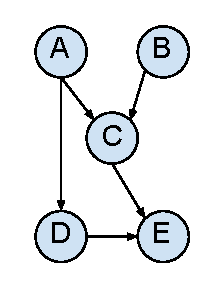
\includegraphics[width=\textwidth]{images/Graph_to_explain_gene_knockout.pdf}
        \caption{ Toy gene regulatory network for wild type i.e. without any knockouts }
        \label{fig:pre_knockout}
    \end{subfigure}
    \begin{subfigure}[b]{0.3\textwidth}
        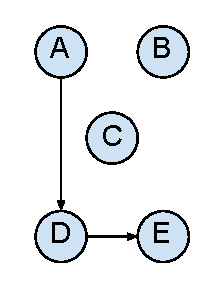
\includegraphics[width=\textwidth]{images/Graph_2_to_explain_gene_knockout.pdf}
        \caption{Same toy gene regulatory network, but where gene C is knocked out}
        \label{fig:with_knockout}
    \end{subfigure}
    \caption{ As an example of a gene knockout experiment, consider the toy gene regulatory network in \ref{fig:pre_knockout}. When we knock out vertex C, it corresponds to cutting all incident and outgoing edges of C. }
    \label{fig:explanation_knockout}
\end{figure}
An additional operation is adjusting the initial values based on the values for the input. In contrast with the previous operation, these values are not kept stationary in subsequent timesteps of a simulation, but they will be 
updated as specified in section \ref{sec:update}.
\subsection{Initial values for the network}
For the initial values of the vertices, we took two different approaches. For the first approach we took two datasets\cite{brauer2008coordination,brauer2005homeostatic} that investigate gene expressions before, during and after
the diauxic shift and used the normalized starting values as the initial values. The second approach consisted of a probabilistic/statistical approach. We  extracted the gene expression levels
for yeast under many different environments from \cite{faith2008many}. Based on these values we estimated the marginal distributions of the genes by fitting them to different continuous probability distributions and selecting the fit that has the lowest
Bayesian information criterion\footnote{$BIC = -2 \ln L + k \ln(n)$ where $L$ is the maximized value of the likelihood,
$n$ is the number of data points and $k$ is the number of free parameters.} value. Based on previous studies 
regarding the continuous distributions of genes \cite{NEEDED} only the Weibull, Gaussian and Gamma distributions were
considered. 
\section{Metabolic Network}
\subsection{Introduction}
A metabolic network consists of all cellular biochemical reactions catalyzed by enzymes as together they form interconnected metabolic pathways
and as such a network. The vertices are called metabolites, which comprises all intermediates or products that in the metabolism of an organism.
\subsection{Dynamic flux balance analysis}
``In flux balance analysis, one constrains the metabolic network by the balance of metabolic fluxes around metabolites. 
When the metabolic network is operating in a steady state, the mass balance is described by a set of linear equations.''
\cite{mahadevan2002dynamic}
When the batch time is divided into several time intervals and the optimization problem is solved at the beginning of 
each time interval, one can get a dynamic solution for the metabolic fluxes. The results are then integrated over the intervals.
\section{Interaction between GRN and Metabolic Network}\label{sec:fba}
Thus far the GRN and metabolic network have only been discussed separately from eachother, but it's possible to combine
them. The GRN contains several nodes that are actually metabolites and therefore values obtained by the flux balance analysis
can be fed to the GRN. Additionally, the metabolic network contains information about what genes are influencing what
chemical reactions. Dependent on the value of those genes, the optimization problem can be redefined by adapting the 
relevant maximal fluxes. 
To map the values of the network from the ranges $[-1,1]$ to $[0,1]$, we feed the gene values to a parametrized logistic function.
% Figure \ref{fig:simulator} shows at a high level how the simulator is composed and what the inputs
and outputs of the systems are. Additionally, pseudocode of the simulator is available at \ref{alg:combi_simulator}.
\begin{figure}	
    \centering
    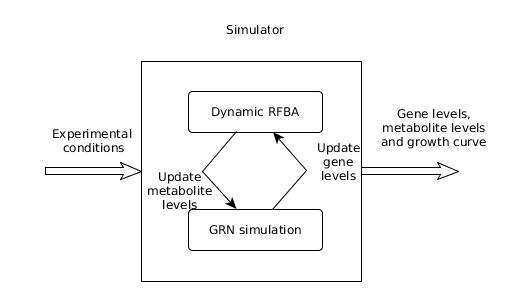
\includegraphics[width=0.4\textwidth]{images/simulator.png}
    \caption{ Illustration of the inputs, outputs, networks and dynamics of the simulator. }
    \label{fig:simulator}
\end{figure}
\begin{algorithmic}\label{alg:combi_simulator}
  \Function{ simulation }{ experiment, initialVertexValues, modelParameters } 
  \Require experiment, initialVertexValues, modelParameters
  \State metabolicModel, geneRegulatoryModel $\leftarrow$ initialize\_networks( modelParameters )
  \State metaboliteValues[0] $\leftarrow$ initializeVertices(metabolicModel, geneRegulatoryModel, initialVertexValues)
  \State adaptWithExperiment(metabolicModel, geneRegulatoryModel, experiment)
  \For{ time in 0:experiment.totalTime }
  \State geneValues[time+1] $\leftarrow$ grnSimulation( geneRegulatoryModel, metaboliteValues[time] )
  \State metaboliteValues[time + 1], growth[time + 1] $\leftarrow$ metabolicSmulation( metabolicModel, geneValues[time+1] )
  \EndFor \\
  \Return growth, geneValues, metaboliteValues
  
  \EndFunction 
\end{algorithmic} 

\section{Probabilistic Estimates}
As typically, there are different sources contributing to uncertainty. The simulator was extended to allow to express different aspects of this uncertainty: initial levels of vertices, model parameters, experimental values.
Currently we only allow specification by means of a (continuous) uniform, Gaussian or Beta distribution, however we can easily extend this to other, both continuous as discrete, distributions.	
Additionally, a combination of deterministic and probabilistic information is still possible: for instance if we are certain that knocking out a gene completely disables the corresponding vertex, the vertex can be completely cut out. However if
there could be a small non-zero value associated with that vertex, it might be more suitable to model it by means of a probability density function. The 
\section{Results}
\subsection{Results of estimates for gene regulatory network}
\subsubsection{Data}
Available datasets can typically be divided in two types: time-course experiments to observe changes in expression levels over time and perturbation experiments to observe effects of a change or treatment on a cell. Since our interest with 
regard to the gene regulatory network lies on the temporal behaviour of gene regulation i.e. the dynamical behaviour, we only selected timeseries datasets from SGD\footnote{http://www.yeastgenome.org/download-data/expression}. We did not 
limit ourselves to datasets solely concerning diauxic shift as we assume that the genetic influences can be averaged over the different conditions. 
This resulted in the following subset: \cite{brauer2005homeostatic,spellman1998comprehensive,cho1998genome,derisi1997exploring,lee2000arrest,carmel2001role}.
Prior to regression tasks, the datasets were normalized (independently from eachother) such that all expression values are contained in the interval $[-1,1]$.%http://libsleipnir.bitbucket.org/Normalizer.html
We obtain appropriate datasets by choosing a $t_{defined}$ and only selecting those datapoints for which we have data of $\Delta t = t_{defined}$. As the datasets are very diverse in their timescales, this results less available data per reaction. These time 
difference are expected to have a significant effect on the output. This resulted in datasets for which the summary can be found in table \ref{tab:summary_time_datasets}.
\begin{table}[htb]
	\centering
   % \resizebox{0.3\textwidth}{!}
   % {
    \begin{tabular}{llll}
    \hline
$\Delta t$(min)&Min&Max&Mean\\
\hline
10&37&94&82.14\\
15&58&111&101.91\\
20&7&53&44.42\\
30&86&170&153.04\\
60&70&136&121.32\\
120&22&52&46.68\\
180&11&31&27.95\\
    \hline
    \end{tabular}
  %  }
    \caption{ Summary of amount of datapoints available per reaction for different time differences. Reported are the minimum amount of data for a reaction, the maximum amount and the average amount. }
	\label{tab:summary_time_datasets}

\end{table}
\subsection{Results of estimates for gene regulatory network}
We trained both a linear support vector regressor and one with an RBF kernel\footnote{with hyperparameter values $C \in \{ 2^k \forall k \in [-10,15[ : k \in \naturalspace \}$ and 
$\epsilon = \{0,0.01,0.05,0.1,0.15,0.2\}$ and L1 loss function} as specified in section \ref{sec:update}.
The results are summarized in table \ref{tab:summary_v_1}, which shows different qualitative measures for the different regressors and for the different time discretizations, but for more clarity only the best time discretizations are shown.
After the hyperparameters were determined by 10-fold crossvalidation, the regressor was retrained with the whole training set. Reported results are on a separate testset, divided in two 80\%-20\% disjoint sets (respectively training and test set).
The linear version is better than the RBF SVR, suggesting that a linear approximation is not necessarily a bad approximation. As a starting network for further optimization, we will therefore use the parameters obtained from the linear support vector
regressor with the discretization of 30 minutes.
Subsequent gene levels are calculated by the following formula:

\begin{equation}\label{eq:gene_update}
 g_v[t+1] = \sum_{j : g_j \in Pa(g_v) \cup \{g_i\} } \theta_{e,(i,j)}g_j[t] + \theta_{v,i}
\end{equation}
\begin{landscape}
\begin{longtable}[htb]{|l|l|l|rrrrr|}

    \hline
Learner& $\Delta$t&Type&Min&Max&Mean&Stdev&Median\\ \hline
\multirow{14}{*}{SVR\textsubscript{Linear}}&\multirow{4}{*}
{20 min}
&MAE&0.0159&0.2879&0.0867&0.0016&0.0779\\
&&MSE&0.0003&0.1612&0.0158&0.0003&0.0099\\
&&MedAE&0.0139&0.2435&0.0687&0.0014&0.061\\
&&$R^2$&-20.5604&0.9725&0.2555&2.8958&0.6092\\
\cline{2-8}
&\multirow{4}{*}{30 min}
&MAE&0.0378&0.4082&0.0879&0.0012&0.0823\\
&&MSE&0.0025&0.2411&0.0161&0.0003&0.0121\\
&&MedAE&0.0217&0.3196&0.0683&0.0009&0.0627\\
&&$R^2$&-1.6544&0.8871&0.4311&0.1062&0.4944\\

\cline{2-8}
&\multirow{4}{*}{60 min}
&MAE&0.027&0.2427&0.0971&0.0012&0.091\\
&&MSE&0.0018&0.1156&0.0198&0.0003&0.0154\\
&&MedAE&0.0217&0.1986&0.0715&0.0009&0.0656\\
&&$R^2$&-1.1329&0.8619&0.3672&0.0997&0.4185\\
\hline
\multirow{14}{*}{SVR\textsubscript{RBF}}&\multirow{4}{*}{20 min}
&MAE&0.0157&0.241&0.0895&0.0014&0.0827\\
&&MSE&0.0004&0.0907&0.0147&0.0002&0.0098\\
&&MedAE&0.0058&0.2366&0.0761&0.0012&0.0716\\
&&$R^2$&-129334.1088&0.9561&-397.5627&51468962.4212&0.6484\\
\cline{2-8}
&\multirow{4}{*}{30 min}
&MAE&0.04&0.2983&0.0851&0.001&0.0786\\
&&MSE&0.003&0.1682&0.0145&0.0002&0.0106\\
&&MedAE&0.0235&0.2722&0.0675&0.0008&0.0632\\
&&$R^2$&-1.1632&0.8885&0.4661&0.0769&0.5155\\
\cline{2-8}
&\multirow{4}{*}{60 min}
&MAE&0.0459&0.262&0.0949&0.0009&0.0897\\
&&MSE&0.0033&0.1309&0.0178&0.0002&0.0143\\
&&MedAE&0.0272&0.2283&0.0737&0.0008&0.0687\\
&&$R^2$&-3.792&0.8471&0.3839&0.1352&0.4388\\
\hline
    \caption{Summary of the results for the learned regressors for the updating function as described in section \ref{sec:update} }
	\label{tab:summary_v_1}
\footnotesize
\end{longtable}
\end{landscape}


\subsection{ Results of combined model }

\chapter{Simulation-based optimization}
\section{Introduction}
In chapter \ref{chap:sim}, we discussed what the simulator is composed of and how it predicts growth curves for gene knockout experiments. This chapter will handle how
the simulator is used to improve the growth curve predictions of the initial model. In order to test the optimization algorithm, we identified different scenarios which we will 
discuss in the next sections. 
% \section{Model parameter estimation}
% %Simulator based optimization
% \cite{ud2015optimal}
\section{Different scenarios}
Recall from chapter \ref{chap:sim} that the simulator actually consists of a gene regulatory network and a metabolic network. From the point of view of our application,
we are primarily interested in learning the gene regulatory network. The different scenarios are related to what the actual output is and thus what can actually be used
in the optimization problem. In every case the simulator takes as input a knockout experiment, which we will call $\mathbf{exp}$. Additionally we will denote the number of
vertices with $N$ and the number of timesteps $T$.
\subsection{Scenario 1: all gene values at every time step}
In this case the output of the simulator exists of the values of every vertex in the graph at every timestep.
This means the simulator is characterized by, $sim_{1}: \mathbf{exp} \to \mathbb{R}^{N \times T}$. This corrresponds to the case where the GRN (only) contains genes and
where an experiment is performed using microarrays.
\subsection{Scenario 2: the values of a subset of gene at every time step}
Compared to the first scenario, the only difference lies in the fact that instead of using all the vertices in the graph, we can only see a subset of them. This could correspond
to learning a gene regulatory network from microarray experiments for which we cannot see all the concentrations, for instance because there are non-gene vertices.
$sim_{2}: \mathbf{exp} \to \mathbb{R}^{N_{sub} \times T}$, with $N_{sub} \subset N$.
\subsection{Scenario 3: one value per time step obtained by applying some function on gene values}
Instead of the values of the vertices being available at every time step, the values are now aggregated in a function that maps the values to a single value at every time step, $f: \mathbb{R}^{N} \to \mathbb{R}$.
By doing so, the simulator creates a single time series instead of one per vertex in the network. The simulator is the transformed into: $sim_{3}: \mathbf{exp} \to \mathbb{R}^{T}$. 
These functions, that operate as proxies for the FBA, were chosen from typical benchmark problems in optimization theory. In the following descriptions of the different functions, we will denote the output as
$out[t]$, similar to before, $g_i$ denotes the value of the $i$-th vertex and $N$ the amount of vertices in the graph.
% \begin{itemize}
%  \item 
% \end{itemize}
% \subsection{Functions} \label{subsec:funcs}
\subsubsection{Summation}
\begin{equation}
 y[t] = \sum_{i=1}^N g_i[t]
\end{equation}
\subsubsection{Summations of squared values}
\begin{equation}
 y[t] = \sum_{i=1}^N g_i^2[t]
\end{equation}
\subsubsection{Rosenbrock function}
\begin{equation}
 y[t] = \sum_{i=1}^{N-1}[100(g_{i+1}[t] - g_i^2[t])^2 + (g_i[t] - 1 )^2]
\end{equation}
\subsubsection{Styblinski–Tang function}
\begin{equation}
 y[t] = \sum_{i=1}^n g_i^4[t] - 16g_i^2[t] + 5g_i[t]
\end{equation}
\subsection{Scenario 4: one value per time step, obtained with FBA}
The results of the metabolic genes are fed to the metabolic network by adjusting the corresponding flux rates and the resulting metabolite fluxes are passed to the metabolic vertices in the gene regulatory network
as described in section \ref{sec:fba}.
% \cite{varma1994stoichiometric}
% \cite{hoffner2013reliable}
% \cite{gomez2014dfbalab}
% \cite{chandrasekaran2010probabilistic}
% \cite{colijn2009interpreting}
\section{Parameters}\label{sec:params}
There are two different sets of parameters that can be optimized, those related to the GRN and those related to the metabolic network. In scenarios 1 to 3, only the GRN parameters are to be optimized, in scenario 4 
both sets. A short description of these is provided in the next sections.
\subsection{GRN parameters}
Previously, we already discussed that the simulator's gene regulatory network has parameters associated with their vertices and edges.
Given equation \ref{eq:gene_update}, we can define a matrix of parameters related to the adjacency matrix of the underlying network:
\begin{equation}
\mathbf{W} = \begin{bmatrix} 
\theta_{e,(1,1)} &\cdots & \theta_{e,(1,N)}\\
\vdots & \ddots & \vdots \\
\theta_{e(N,1} & \cdots & \theta_{e,(N,N)} 
      \end{bmatrix}
\end{equation}
% \boldsymbol{\theta_e}, \boldsymbol{\theta_v}
and

\begin{equation}
 \boldsymbol{\theta_v} = \begin{bmatrix}
     \theta_{v,1} \\
      \vdots \\
      \theta_{v,N} 
     \end{bmatrix}
\end{equation}

Where $\theta_{e,(i,j)}$ is non-zero if there is a directed edge from vertex $i$ to $j$ and the value being the influence that vertex $i$ has on $j$ and $\theta_{v,i}$ is a constant term indicating the behaviour on the level of a vertex $i$ 
when there is no interaction (i.e. the incoming nodes have level 0) cfr. equation \ref{eq:gene_update}. This gives us the following vector of parameters:
\begin{equation}
 \mathbf{\theta} = \begin{bmatrix}
                     \theta_{e,(1,1)} \\
                     \vdots \\
                     \theta_{e,(N,N)} \\
                     \theta_{v,1} \\
                     \vdots \\
                     \theta_{v,N}
                    \end{bmatrix}
% 
\end{equation}
\subsection{Metabolic network parameters}
Additionally we parametrized how the gene regulatory network interacts with the metabolic network similar by adjusting the fluxes 
by incorporating gene expression levels as in \cite{chandrasekaran2010probabilistic}.
As the gene regulatory network generates continuous values, we apply
a logistic function to map these to the interval $[0,1]$. 
In the equation of the logistic curve 
\begin{equation}
 f(x) = \frac{L}{1+e^{-k(x-x0)}}
\end{equation}
there are different parameters that need to be set: $L$, $k$ and $x0$, so for every gene that influences the metabolic
network there are 3 additional parameters. The metabolic network contains a total of 904 genes\footnote{In the metabolic model iMM904}, whereas the gene regulatory
network for diauxic shift contains 333 genes. Taking the intersection of those two sets yields a total of 146 genes
% \footnote{These are: YBL015W, YLR304C, YJL200C, YAL054C, YLR153C, YOL086C, YMR303C, YMR083W, YBR145W, YCR010C, YCL025C, YBR132C, YMR169C, YOR374W, YER073W, YPL061W, YPR128C, YBR149W, YOR377W, YDR384C, YPL111W, YLR438W, YML042W, YOR125C, YAL038W, YNR001C, YCR005C, YPR001W, YHR051W, YOR100C, YDR256C, YGR088W, YML054C, YJR048W, YJL005W, YOR065W, YML070W, YIR029W, YIR032C, YIR028W, YJR152W, YIR031C, YOR180C, YDL174C, YEL071W, YBR208C, YHL016C, YLR284C, YGR254W, YHR174W, YOR317W, YER015W, YMR246W, YKL060C, YLR377C, YOR388C, YKR009C, YLL043W, YPL262W, YAL062W, YCL040W, YDL022W, YKL152C, YDL021W, YDR098C, YHL032C, YIL155C, YER062C, YFR053C, YGL253W, YHR094C, YMR011W, YDR345C, YHR092C, YHR096C, YDR343C, YDR342C, YER065C, YPR006C, YNL037C, YOR136W, YDL066W, YLR174W, YNL009W, YKL217W, YIL125W, YDR148C, YFL018C, YOR142W, YGR244C, YKL029C, YKL085W, YOL126C, YDL078C, YNL117W, YML120C, YKR097W, YLR044C, YLR134W, YGR087C, YGL248W, YOR360C, YGR240C, YMR205C, YIL107C, YOL136C, YBR196C, YCR012W, YKL127W, YMR105C, YMR006C, YIL160C, YGL205W, YPL147W, YKL188C, YGL062W, YBR218C, YOR347C, YJL166W, YKL148C, YLL041C, YKL141W, YDR178W, YOR184W, YJR095W, YNL202W, YDR536W, YPL057C, YJL052W, YJR009C, YGR192C, YJR019C, YBR117C, YJR066W, YKL203C, YDR050C, YBR126C, YDR074W, YGR019W, YBR006W, YDL210W, YEL021W, YAR035W, YER024W, YJL045W, YNL241C}
The metabolism of yeast is well understood, at least better than the gene regulatory network\cite{NEEDED}. For this reason we primarily parametrize the gene regulatory network and how it interacts with the metabolic network
and leave the metabolic network as is.
\section{Optimization problem}
\subsection{Introduction}
In this section we will discuss several aspects of the optimization problem. This includes the optimization algorithm, adjustments of the standard algorithms, tunable parameters and objective functions.
\subsection{Gradient descent}%http://link.springer.com/chapter/10.1007%2F978-3-642-35289-8_25#page-1
Gradient descent is an optimization method that tries to optimize an objective function by iteratively updating the parameters of its model.
In gradient descent the parameter vector is updated iteratively by calculating the gradient at a certain point and updating the weights in the direction of the negative gradient as this is the direction in which the function is declining. 
In regular gradient descent the calculation of the gradient is done on the whole training set. Given a multi-variable function and parameter vector $\mathbf{x}$
$F(\mathbf{x})$ and if it is defined and differentiable in a certain point $\mathbf{a}$, and given a
certain learning rate $\gamma$  the new point $\mathbf{b}$ is calculated as follows.
\begin{equation} \label{eq:gd}
 \mathbf{b} = \mathbf{a} - \gamma \nabla F(a)
\end{equation}
 \subsection{Stochastic Gradient Descent} 
 Stochastic Gradient Descent(SGD) is a simplification of the Gradient Descent(GD) algorithm. Whereas GD updates the parameter vector by calculating the gradient for all training examples, SGD estimates
 the gradient based on a single randomly picked example, resulting in a noisier approximation of the gradient.
%   <POPULARITY>
  
 \subsection{Objective Function}\label{section:obj}
 Recall that equation \ref{eq:gd} requires us to specify some function $F(\mathbf{x})$ whose value will be minimized. For this work, we employed the Mean Squared Error. As the outputs for the different scenerios
 are not the same, there are some differences in the equations which we will quickly discuss.
 \subsubsection{Scenario 1}
 \begin{equation}
  F_{1}(\mathbf{x}) = \frac{1}{N\cdot T} \sum_{i=1}^N\sum_{t=1}^T(\hat{y}_i[t] - y_i[t])^2
 \end{equation}
 where N is the total amount of values, which is the amount of genes multiplied with the amount of time steps, $i$ iterates
 over all these values, $\hat{y}_i$ is the value estimated by the model and $y_i$ is the actual value.
 \subsubsection{Scenario 2}
 \begin{equation}
  F_{2}(\mathbf{x})  = \frac{1}{N_{sub}\cdot T} \sum_{i=1}^{N_{sub}}\sum_{t=1}^T(\hat{y}_i[t] - y_i[t])^2
 \end{equation}
 In this case only a subset $N_{sub} \subset N$ of the vertices is used .
 \subsubsection{Scenarios 3 \& 4}
 \begin{equation}
 F_{3,4}(\mathbf{x}) = \frac{1}{T} \sum_{t=1}^T(\hat{y}[t] - y[t])^2
 \end{equation}
 with $y[t]$ and $\hat{y}[t]$ denote respectively the actual and estimated output of the aggregate function or of the growth curve obtained from FBA at time $t$.
 
\subsection{Gradient of objective function}
In fact, it's not the objective function itself which is needed for the gradient descent algorithm, but rather the gradient of the objective function. If analytical solutions of the derivates
are available, it is better to apply them directly. In some cases however it is not possible to obtain these analytical solutions. In our application this would involve obtaining a closed-form solution
to the optimization problem defined by flux balance analysis, which at the very least is not straightforward. The simplest way to numerically approximate the gradient is the technique of finite differences. 
The approximation consists of obtaining the values for the objective function where a \textit{small} number is added and subtracted for every parameter separately and then dividing the difference of them by two times the \textit{small} number.
This approximation is however highly numerically inefficient as this requires an amount of function evaluations equal to two times the size of the parameter vector.
On the other hand, in simultaneous perturbation stochastic approximation(SPSA)\cite{hazen2009gradient} the gradient is estimated by stochastically choosing a direction
in which to perturb the operating point to calculate a finite difference gradient. 

\begin{equation}
 \hat{\nabla f(c)}[d] = \frac{f(x_k + \delta_k\Delta_k[d]e_d) - f(x_k - \delta_k\Delta_k[d]e_d)}{2\delta_k\Delta_k[d]}
\end{equation}
``where $e_d$ is a $D$-component vector with 1 for the $d$th component and 0 for all other components, $\delta_k$ is a 
scalar that generally shrinks as the number of iterations $k$ increases, and $\Delta_k$ is a random $D$-component perturbation
vector."
This approach only requires 2 evaluations of $f$ to calculate a gradient.
%  SPSA \url{http://www.jhuapl.edu/spsa/}
%  SAA \url{https://people.orie.cornell.edu/shane/pubs/SAAGuide.pdf} sample average approximation, \url{http://www.stat.columbia.edu/~liam/teaching/compstat-spr15/lauren-notes.pdf}

 
\subsection{Learning rates}
It is possible to keep the learning rate $\gamma$ from equation \ref{eq:gd} fixed throughout the different iterations, however previous studies have shown that improved convergence can be obtained by allowing
$\gamma$ to be altered in subsequent iterations \cite{jacobs1988increased}. These techniques are however still sensitive to the initial choice of the learning rate. A (relatively new) technique called AdaDelta\cite{zeiler2012adadelta}
avoids choosing and having to manually tune a learning rate altogether and good results for this adaptive schemes have been reported. An overview of the revised algorithm is shown in figure \ref{fig:adadelta}.
% \subsection{AdaGrad}
% \cite{duchi2011adaptive}
\begin{figure}	
    \centering
    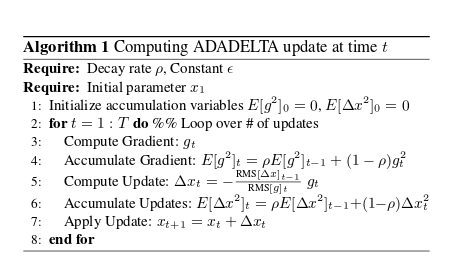
\includegraphics[width=0.4\textwidth]{images/ada_delta.png}
    \caption{ An overview of the AdaDelta algorithm. }
    \label{fig:adadelta}
\end{figure}

\subsection{Stopping mechanism}
To avoid overfitting an early stopping mechanism is applied on a whithheld validation set. If the performance does not improve for 50 iterations, the algorithm is terminated and returns the best parameter vector before those 50 iterations.
There is also a maximum on the amount of iterations: if this maximum is reached, the algorithm also stops even though the optimization process might still be improving the parameter vector.
% 
% \subsection{Model Space}
% % http://onlinelibrary.wiley.com/doi/10.1111/j.2041-210X.2012.00236.x/full :
% % Simulations or observations of flow dynamics occurring on networks with fixed topology can be described using time-ordered networks (Table 1, F4, C2). For a network with fixed topology whose edges represent potential interactions that depend on the details of the system, the occurrence and ordering of actual interactions can be completely described by a time-ordered network. The approaches described in previous sections can then be used to make time-dependent descriptions and inferences about the system. This approach may also be valuable for individual-based or cellular automata models (Wolfram 2002) where network topology is fixed – for example, in a cellular automata model of pollen flow between multiple patches with unchanging connectivity, one could simulate the activity of different pollen carriers and test the hypothesis that plants with more conspecific neighbours had higher rates of resource flow. An area of active application is in social learning, where network-based diffusion analysis (Franz & Nunn 2009; Hoppitt, Boogert & Laland 2010) is used to assess how the social structure of a group predicts the rate of acquisition of a new behaviour in group members. This general approach of fitting multiple competing models of flow on a fixed network to observed patterns of flow would likely be applicable in other areas.
% Different application: graph is a structure of roads, output is amount of kms of traffic jam, try to find influence of particular crossroads wrt the traffic jam.
%  Influence propagation in social network with output being popularity of product over time? cfr product life cycle curve.
%  \subsection{Related work}
%  \cite{costa2014rbfopt} black box optimization with gaussian processes, \cite{amaran2014simulation} simulator optimization (no focus on optimizing parametried graphical structure of simulator from proxy)
%  \cite{raza2014recurrent}.
 \section{Experiments}
 \section{Introduction}
 This section will cover some aspects about the experiments that we perform with the optimization algorithm such as
 how the the datasets were generated or obtained, how we evaluate the results. 
 \subsection{Datasets}
 \subsubsection{Toy datasets}
 We considered two types of networks, complete digraphs\footnote{``A complete digraph is a directed graph in which every pair of distinct vertices is connected by a pair of unique edges (one in each direction).''} and scalefree networks
\footnote{``A scale-free network is a network whose degree distribution follows a power law, at least asymptotically.That is, the fraction P(k) of nodes in the network having k connections to other nodes goes for large values of k as 
$ P(k) \sim k^{-\gamma} $ where $\gamma$ is a parameter whose value is typically in the range $2 < \gamma < 3$ \cite{barabasi2004network}, although occasionally it may lie outside these bounds''}. We have opted for this
kind of networks as a lot of real-life networks can be characterized as being scalefree. Examples of such graphs include biological networks such as gene regulatory networks and protein interaction networks, social networks and more \cite{barabasi2009scale}
The parameters related to the vertices and edges are randomly sampled from the normal distribution with mean $0$ and standard deviation $1$. Given this network we then generated a list of all possible knockout experiments(input to the system), and
calculated the outputs with this network and the simulator, adding different levels of noise. These toy datasets were then used for scenarios 1, 2 and 3.
 \subsubsection{Eve Growth curves}
 Currently not available.. Needed for scenario 4.
 \subsection{Evaluation}\label{sec:eval} 
To evaluate the output of the parameter estimation algorithm we calculate the mean squared error on a separate testset (see Section \ref{section:obj}) and the Euclidian distance of the optimal
parameter vector to the real parameter vector (see Section \ref{sec:eval}). When using the output of the optimization algorithm as samples we use the kolmogorov-smirnov statistic rather than
the Euclidian distance.

% \subsection{Parameters}
% Parameters either deterministic or probabilistic, 
% using an ensemble of learners to estimate probabilistic parameters \cite{carney1999confidence}.
% \subsection{Experiments}
% 
% Parameters of vertices (cfr. infra \ref{sec:params}) are sampled from the normal distribution $\mathcal{N}(0,1)$
%    
% We tested the following scenario's:
% \begin{itemize}
%  \item Every value of every vertex is available for every time step
%  \item Every value of a subset of vertices is available for every time step
%  \item At every timestep the values of the vertices at that timestep is used to calculate one single value for that timestep. These
%  functions are explained in \ref{subsec:func}.
% \end{itemize}
Every set of algorithmic parameters is repeated 10 times with different randomized networks. The length of the time series is kept at 10.


\subsection{Results}
% output from script in validation\_scripts,  test\_functions, test\_functions2 and test\_functions3
% 03 of august, new runs (\url{AdaLab/validation_script/to_run})
% \begin{verbatim}
% % pinac 25: test_functions.sh and test_functions_adadelta.sh
% % pinac 26: test_functions_2.sh and test_functions_2_adadelta.sh
% % pinac 27: test_functions_3.sh and test_functions_3_adadelta.sh
%  
% \end{verbatim}
    
%%Dynamic neural networks feed back output and use it as (part of) the input typically 
%%Dynamic neural networks not only deal with nonlinear multivariate behaviour, but also include (learning of) time-dependent behaviour such as various transient phenomena 
%%and delay effects. Techniques to estimate a system process from observed data fall under the general category of system identification.
%%Recurrent neural networks: Contrary to feedforward networks, recurrent neural networks (RNNs) are models with bi-directional data flow. 
%%While a feedforward network propagates data linearly from input to output, RNNs also propagate data from later processing stages to earlier stages. RNNs can be used as general sequence processors.
%Stochastic approximation http://castlelab.princeton.edu/ORF569papers/Powell%20ADP%20Chapter%206.pdf 
%Stochastic optimization http://www.stat.columbia.edu/~liam/teaching/compstat-spr15/lauren-notes.pdf
%Use NetGenerator V2.0?	

\bibliographystyle{plain}
\bibliography{simulator_optimization}

\end{document}